\documentclass{IEEEtran}
\usepackage{amsmath,amssymb,amsfonts}
\usepackage{algorithmic}
\usepackage{graphicx}
\usepackage{textcomp}
\usepackage[OT1]{fontenc}


\usepackage[style=numeric-comp]{biblatex}
%\RequirePackage[style=numeric,doi=false,isbn=false,url=false, firstinits=true, maxbibnames=99]{biblatex}
\addbibresource{references.bib}

\def\BibTeX{{\rm B\kern-.05em{\sc i\kern-.025em b}\kern-.08em
    T\kern-.1667em\lower.7ex\hbox{E}\kern-.125emX}}

\begin{document}

\title{Comprehensive Overview of V2X Communication Prediction Methods for
Cooperative Vehicular Maneuver Coordination}
\author{M. Nilges}
\thanks{Submitted May 2020. Thanking my supervisor, Daniel Bischoff.}
\thanks{Malte Nilges is student at the Technische Universität Darmstadt (e-mail: malte.nilges@gmail.com). }

\maketitle

\begin{abstract}
    This paper gives a brief overview of the current state of Quality-of-Service (QoS) prediction concepts in the evolving V2X technologies. Firstly, the relevant metrics for intelligent transportation systems are identified for which a prediction proves to be useful. The considered technologies include C-V2X with its key interfaces Uu for cellular communication and PC5 for direct communication between UEs as well as 802.11p.
    
    For these technologies available and considered concepts are presented and a comparison is being drawn.
\end{abstract}

\begin{IEEEkeywords}
V2X, V2V, V2I, V2N, QoS, Prediction, C-V2X, 802.11p, 5G
\end{IEEEkeywords}

\section{Introduction}
\label{sec:introduction}
\IEEEPARstart{I}{}n recent years, proactive communication between vehicles became a more prevalent matter of research. Today many manufacturers try to implement new technology into their vehicles, aiming at  improved security and comfort for the passengers. The needed communication infrastructure is developing fast, with several technologies available to choose from depending on the use case.

One important use case of this new technology is the cooperative maneuver coordination, as this cooperation between vehicles enables an even higher degree of automation, leading to more efficient traffic and safety in complex driving situations.

Independently from the deployment, as a centralized or decentralized approach, this high level of cooperation has strict performance requirements of the communication links. Yet there is no guarantee if these requirements will be satisfied at all times due to poor network coverage or propagation conditions.

As a priori knowledge of the communication quality may serve to adjust and enhance the level of cooperation, this study performs a research in currently available communication prediction methods and evaluates these approaches in terms of their applicability to the use case of autonomous cooperative maneuver coordination.

The paper is structured as follows: First, it will give an overview of related works. Following that, Sect. 3 will introduce the concept of cooperative maneuver cooperation and analyze its requirements on communication. In Sect. 4 current research of prediction methods is being explored. The following discussion will evaluate the existing methods in terms of their applicability on cooperative maneuver coordination and lay the foundation for the conclusion.


\section[]{Related Works}
As this work tries to give a comprehensive overview of prediction methods with a given set of constraints, other works providing overviews of methods or constraits must not be neglected. These can be grouped into different categories based on the research topics they portray.
\subsection{Network Basics}
Existing studies give a great overview of the challenges faced in vehicular communication. While Mecklenbräuer et al, 2011 gives an overview the available technologies, its focus lies in the depiction of the communication channels, the various scenarios (V2V, V2I, cellular), the metrics (e.g. fading, path loss and doppler shift) as well as the models (e.g. raytracing or stochastic models) for their simulation.

For the estimation of the communication channel, traditionally pilot symbols are being used, which contain no data, but by which the receiver is able to estimate and equalize received data. This estimation is the key element in achieving low bit error rates (BER) but not trivial. 

Existing pilot patterns such as the one from 802.11p were not designed for highly mobile networks, thus leading to decreased performance in these scenarios. Some of our the reviewed methods try to take the prediction as an advantage for channel estimation, as such it is crucial to understand and distinct these terms.
\subsection{Communication Prediction}
As by now, efforts in the standardization of vehicular communication prediction are undertaken, the 5GAA summarized the key concept of QoS prediction and its use cases and challenges. Notably, the whitepaper identifies possible deployment methods, namely Over-The-Top and Mobile Network Operator prediction, as well as  

\section{Cooperative Maneuver Coordination}
Cooperative Maneuver Coordination is the aim of making automated vehicles influence the each others behaviour and enabling joint driving maneuvers, making road traffic safer and more efficient.
The concept consists of multiple use cases, among others \cite{bobanConnectedRoadsFuture2018}:
\begin{itemize}
\item lane changing
\item platooning
\item cacc (cooperative adaptive cruise control)
\item intersection control
\item collision avoidance
\end{itemize}
Hereby different approaches exist, either as centralized \cite{mengluICTInfrastructureCooperative2018} or decentralized cooperation \cite{llatserCooperativeAutomatedDriving2019,fortelleNetworkAutomatedVehicles2014}.

In a centralized cooperation, a central entity such as a RSU, gains global knowledge by the usage of its own sensor data and direct communication with the vehicles in its coordination range and thereby plans optimal maneuvers in terms of efficiency and safety.

The decentralized approach does not rely on a central entity, but rather leaves the planning to the vehicles, which adapt their maneuvers based on maneuver intentions shared by surrounding vehicles in order to achieve locally optimal traffic patterns.

Without going too much into the details of implementation methods for the coordination, we rather want to take a look at the aspect of communication. Several works investigated the requirements for the communication links. Typical KPIs (Key Performance Indicators) are end-to-end latency, reliability, data rate (per vehicle) and the communication range.

Boban et al. \cite{bobanConnectedRoadsFuture2018} suggest a latency of sub 3 to 100 ms, a required data rate of 1.3 to 25 MB/s, depending on the degree of sensor data dissemination, and a transmission reliability of over 99\%.

As stated in \cite{llatserCooperativeAutomatedDriving2019}, the number of exchange messages and their contained amount of data need to adapt dynamically in order to prevent channel congestion, as it is apparent that the aforementioned link requirements cannot be met at all times. Furthermore vehicles need to interact with their environment even without these cooperation messages.

The aim of this work is to evaluate existing communication prediction methods in terms of their applicability on the cooperative maneuver coordination. Therefore we first need to identify possible prediction scenarios and use cases.

If we take the use case of intersection control and collision avoidance for example, it is clear, that vehicles are approaching each other from different directions and the requirements on the reliability on the communication between these vehicles are of a higher priority than the communication with other vehicles of the area. While a global prediction is attractive, the close-to-mid range prediction is far more relevant in such use cases. 

The most interesting parameters are the reliability, e.g. measured in packet loss, and latency, as they decide whether the communication is stable enough in order to be used for cooperation. Otherwise the predictions can be used to initiate safety measures such as increased distancing against the desire for perfect efficiency.

\section{Scope of the Paper}
While there are many channel quality prediction approaches, not all are appropriate for our use case.

This paper lays its focus on higher level V2X communication prediction, hence methods aimed at replacing traditional pilot-based channel estimation used for adaptive transmission techniques such as adaptive modulation, channel coding or power control will not be covered.
While these methods may use similar prediction methods (e.g. autoregression and machine learning), they are used for immediate future link level channel prediction.
For further research in this area of research please refer to \cite{semmelrodtInvestigationDifferentFading2003,duel-hallenFadingChannelPrediction2007,wongJointChannelEstimation2005,wongWLC435LowComplexityAdaptive2006,vaughanShorttermMobileChannel2000}


\section{Methods}
Methods for Communication Prediction can be primarily split into two categories, on the one hand the channel quality prediction for the immediate future and on the other hand channel quality or related indicator prediction for the short- to long-term future.

\subsection{Immediate Channel Prediction Schemes}
The immediate channel quality prediction is mainly targeted as an extension resp. an alternative for traditional channel quality estimation using pilot symbols.
Over the years, a large number of works using different prediction algorithms emerged. 

Traditional prediction schemes based on channel propagation models or past channel information can be classified into the three methods: Sum-of-Sinusoids (SOS) Model, Basis Expansion (BE) Model and Autoregression (AR) Model.

Common to these traditional methods is their time frame, predicting only several milliseconds into the future for high velocity nodes. This time frame is small, but enables adaptive transmission techniques such as adaptive modulation, channel coding or power control and even adjustments in high level applications in contrast to using estimated CSI, which is instantaneously outdated at higher velocities.

\subsubsection{AR}
The AR model uses previous channel samples in form of CSI in combination with time-variant coefficients. These channel coefficients need to be computed using estimation techniques, either static, such as Wiener filter or LS criterion, or adaptive, such as various LMS or RLS filters.

One of the most acclaimed works in this area of research was conducted by Duel-Hallen et al. \cite{duel-hallenLongrangePredictionFading2000}. Their research was performed in order to provide a long-range channel prediction algorithm by predicting the channel coefficients up to hundreds of symbols ahead using LMS filtering, which is adaptive and computationally less expensive than RLS filtering.
The method was tested against simulated and measured data of static and mobile environments and yielded improved BER when combined with adaptive channel modulation.

\subsubsection{SOS}
In contrast to AR, the SOS model approximates the physical propagation process by modelling the channel as a linear combination of complex sinusoids. This model provides a good predictive performance, but only in cases where the channel parameters consisting of amplitude and Doppler frequency are static.

Noteworthy are the MUSIC and ESPRIT algorithms used in \cite{wongWLC435LowComplexityAdaptive2006,wongJointChannelEstimation2005,semmelrodtInvestigationDifferentFading2003,tealSimulationPerformanceBounds2001,vaughanShorttermMobileChannel2000,chenNewApproachesChannel2006} where \cite{wongWLC435LowComplexityAdaptive2006} provides a reduced complexity ESPRIT algorithm, that tries to reduce the computational complexity of time-variant parameters seen in realistic channels.

\subsubsection{BE}
The BE model describes the channel as a linear set of basis functions, such as complex exponential (CE) or discrete prolate spheroidal (DPS) sequences, multiplied by coefficients, which are obtained through analysis of the pilot data. Zemen et al. \cite{zemenMinimumEnergyBandLimitedPredictor2007} provide a method based on time-concentrated and band-limited DPS sequences. The predictor dynamically selects the spanned subspace with the smallest reconstruction error and utilizes it in order to predict the channel.


While the DPS-BEM outperforms DPS-CEM in numerical simulations, yet no comparison is concluded against SOS and AR models. Of the latter two, AR models seem to perform better in terms of their prediction horizon and computational complexity as stated in \cite{semmelrodtInvestigationDifferentFading2003}.

\subsubsection{Machine Learning}
\subsection{Short- to Long-Term Prediction Schemes}


The short- to long-term prediction is targeted rather at high-level applications that need long term knowledge for adjusted communication. Therefore predictions are mostly performed for indicators such as throughput, latency or package loss, which are linked to the channel quality.



Zeng et al. [] propose the usage of AR model-based prediction specifically for usage in V2X scenarios, enabling improved centralized scheduling compared to centralized scheduling techniques relying on collected real-time CSI. 
Their solutions is a channel prediction and scheduling scheme using RSUs and Control Servers which receive data for prediction of the best relay candidate of the connected vehicles. The prediction is achieved using current velocity and position which yields the respective distances between the nodes. Using a predetermined LS fading model, a value for the LS fading can be predicted and used in a computation of the SNR. Using that value, a centralized scheduling scheme is applied based on the best candidate.
While this technique reduces the transmission overhead and delay and opens the doors for further use cases of the predictions, the simulations were performed using a static path loss model which doesn’t account for parameters such as refraction or scattering.

\subsubsection{Connectivity Map Based Methods}
We start off the examination of works with so-called connectivity maps as they present the most simple concept for prediction of future connectivity. Mobile nodes such as vehicles share their experienced network quality with a central back end using their data channels, which in turns aggregates all the received data in a map.

This concept differs from the related network coverage maps, which use mathematical models in order to determine network coverage and quality at a given place.
The data aggregated for the connectivity map differs, as well as the processing that is performed when determining the network quality on a given location.

Kelch et al. [] examine this concept in the vehicular application, focusing on the acquisition and matching of data, which includes CQI values queried for generated TCP/IP traffic on their cellular modem, as well as the coordinated gathered by a GPS module. In order to make good predictions for map segments, they examine a map segmentation method called Jump-P [], which outperforms simple fixed length segmentation in terms of the trade-off between the number of needed map segments and the RMSE of the pooled data. The CQI values shared to the sender determine the block size, as better channel conditions allow for a more optimized data transmission, thus enabling an estimation of the theoretical throughput for a given CQI value.

Summarizing, this method enables a prediction of the theoretical throughput by previously collected  CQI values. Only a small range of CQI values lead to tolerably accurate predictions, as values below 20 rarely appeared and values above 25 were exceedingly inaccurate.

A similar approach is performed by Pögel et al. [], but in contrast they are collecting different data in the form of RSSI (which is part of CQI) as well as used cells, actual bandwidth and latency at a given location. This leads to a more accurate prediction, but as the authors show, the accuracy is highly dependant on external factors such as average speeds, congestion and weather as they show in their tests performed on different weekdays. As the map simply delivers collected data, it is not self-adjusting to these external factors.

The only comparable measurement of connectivity maps is performed by Schmid et al. [] predicting the Round Trip Time (RTT) in addition to the throughput. Laying their focus on the segmentation of such a connectivity map, their results showed that even for an optimal manual segmentation, the RMSRE between the measured and predicted values is at least 39.12\% which leads them to conduct history based algorithms in order to predict future throughput.

















\begin{figure}[!t]
\centerline{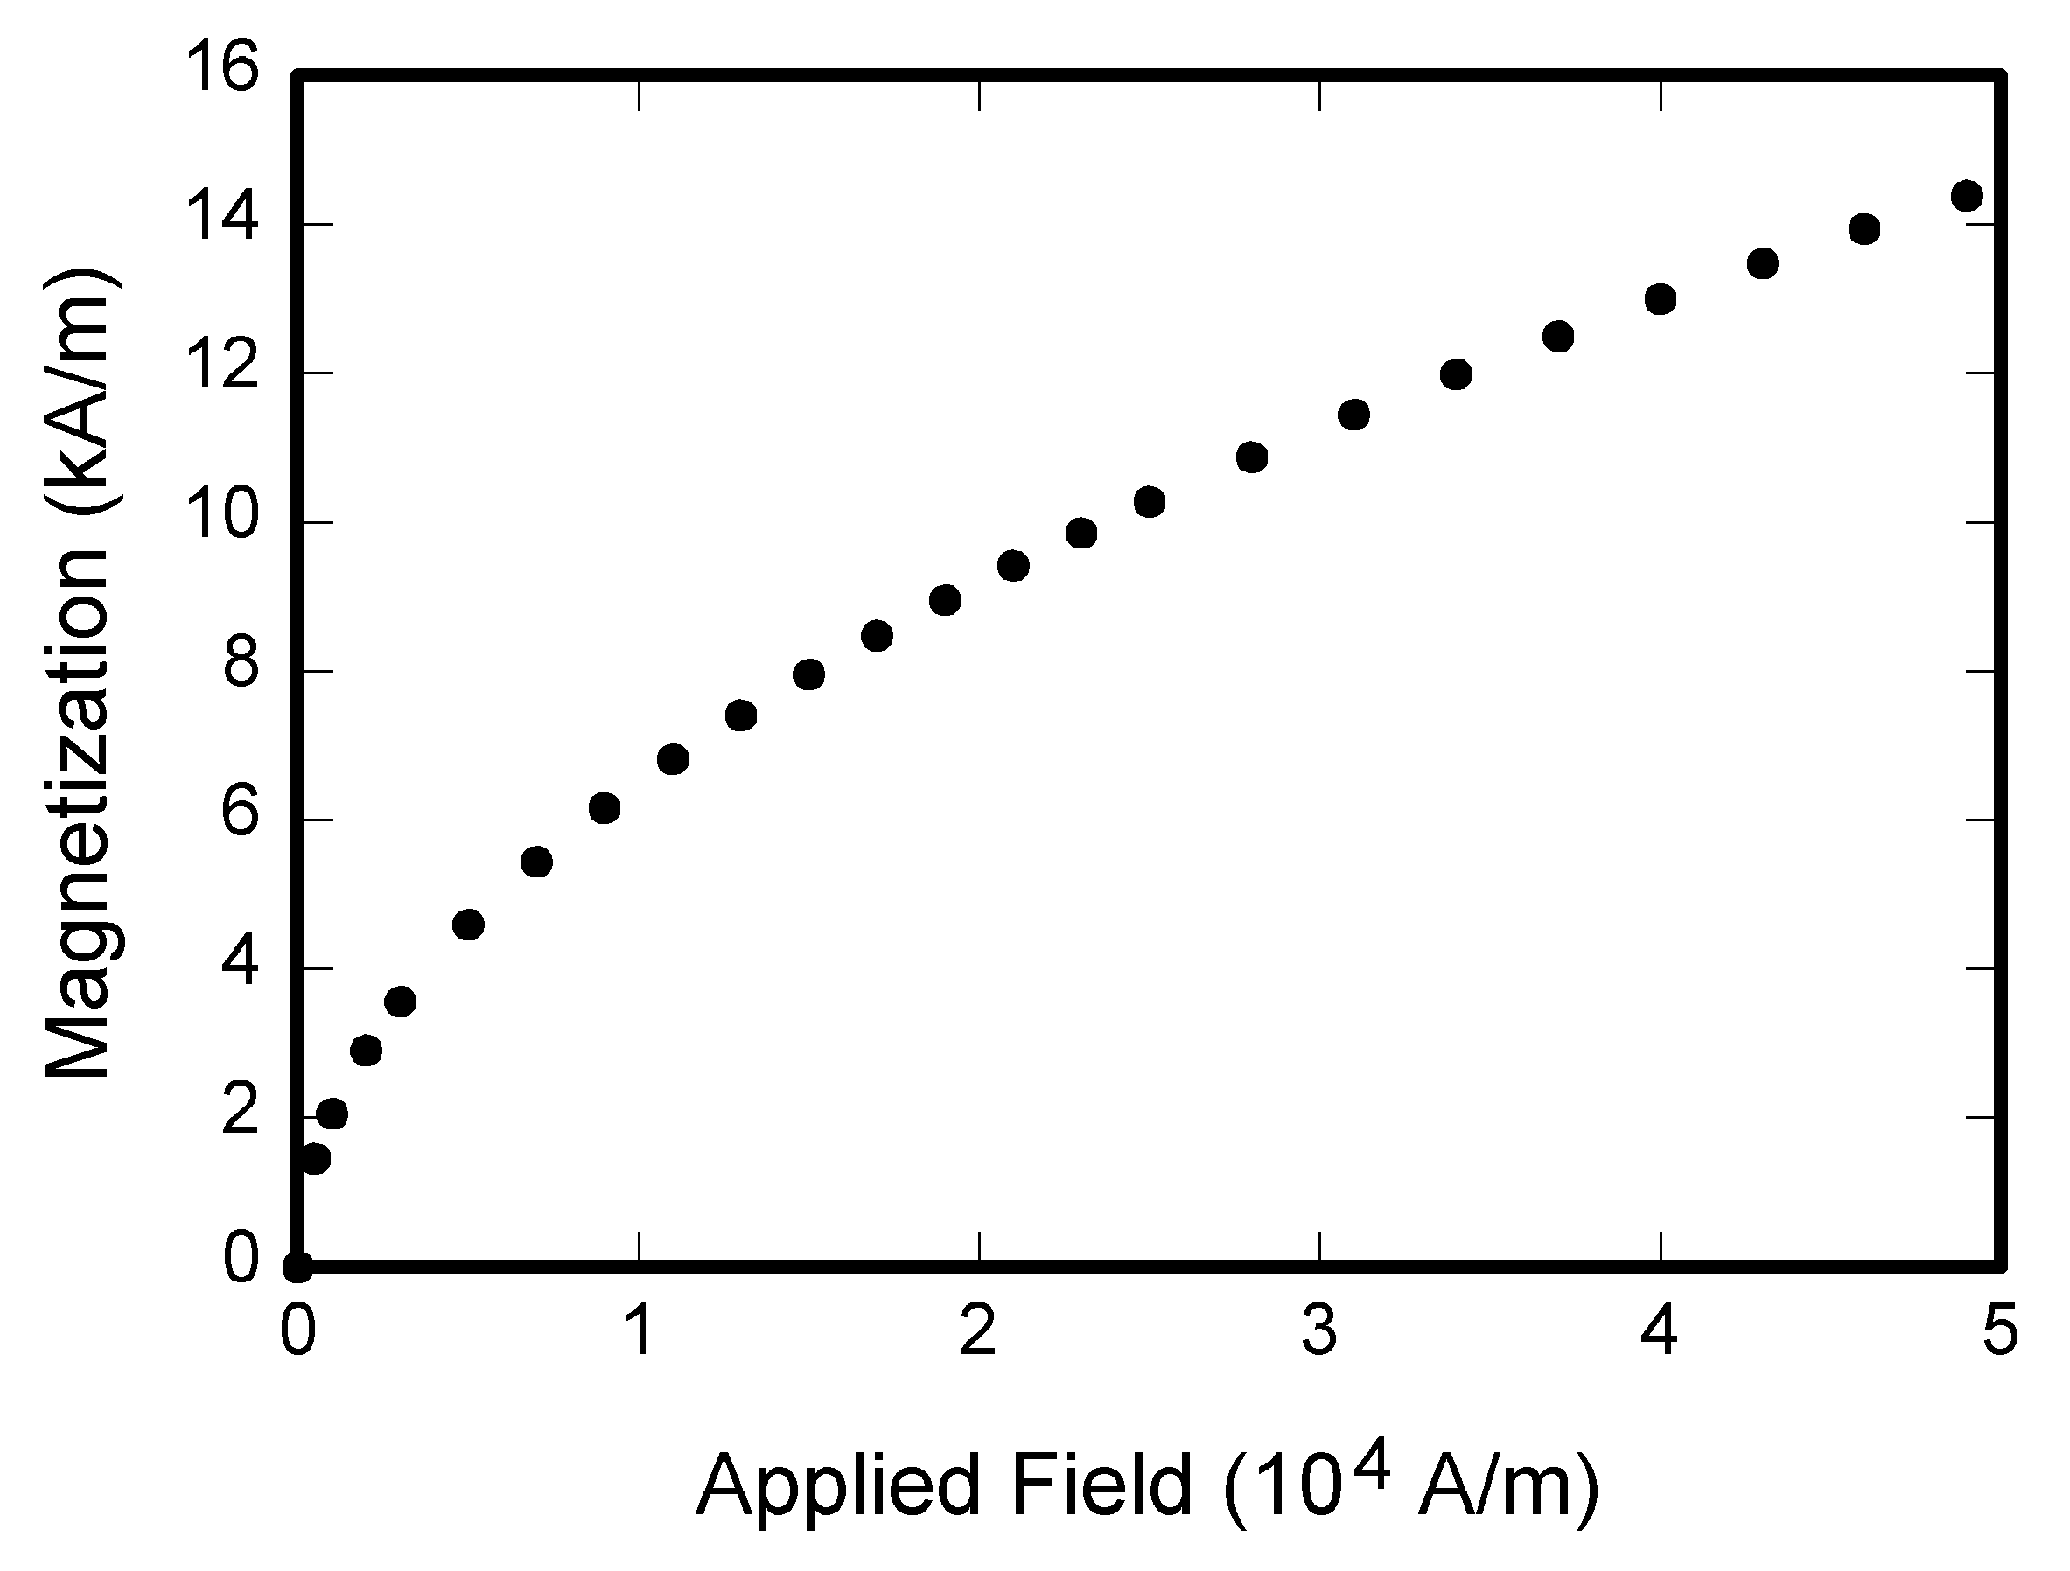
\includegraphics[width=\columnwidth]{fig1.png}}
\caption{Magnetization as a function of applied field.
It is good practice to explain the significance of the figure in the caption.}
\label{fig1}
\end{figure}

Be aware of the different meanings of the homophones ``affect'' (usually a 
verb) and ``effect'' (usually a noun), ``complement'' and ``compliment,'' 
``discreet'' and ``discrete,'' ``principal'' (e.g., ``principal 
investigator'') and ``principle'' (e.g., ``principle of measurement''). Do 
not confuse ``imply'' and ``infer.'' 

Prefixes such as ``non,'' ``sub,'' ``micro,'' ``multi,'' and ``ultra'' are 
not independent words; they should be joined to the words they modify, 
usually without a hyphen. There is no period after the ``et'' in the Latin 
abbreviation ``\emph{et al.}'' (it is also italicized). The abbreviation ``i.e.,'' means 
``that is,'' and the abbreviation ``e.g.,'' means ``for example'' (these 
abbreviations are not italicized).

A general IEEE styleguide is available at \underline{http://www.ieee.org/authortools}.

\section{Guidelines for Graphics Preparation and Submission}
\label{sec:guidelines}

\subsection{Types of Graphics}
The following list outlines the different types of graphics published in 
IEEE journals. They are categorized based on their construction, and use of 
color/shades of gray:

\subsubsection{Color/Grayscale figures}
{Figures that are meant to appear in color, or shades of black/gray. Such 
figures may include photographs, illustrations, multicolor graphs, and 
flowcharts.}

\subsubsection{Line Art figures}
{Figures that are composed of only black lines and shapes. These figures 
should have no shades or half-tones of gray, only black and white.}

\subsubsection{Author photos}
{Head and shoulders shots of authors that appear at the end of our papers. }

\subsubsection{Tables}
{Data charts which are typically black and white, but sometimes include 
color.}

\begin{table}
\caption{Units for Magnetic Properties}
\label{table}
\setlength{\tabcolsep}{3pt}
\begin{tabular}{|p{25pt}|p{75pt}|p{115pt}|}
\hline
Symbol& 
Quantity& 
Conversion from Gaussian and \par CGS EMU to SI $^{\mathrm{a}}$ \\
\hline
$\Phi $& 
magnetic flux& 
1 Mx $\to  10^{-8}$ Wb $= 10^{-8}$ V$\cdot $s \\
$B$& 
magnetic flux density, \par magnetic induction& 
1 G $\to  10^{-4}$ T $= 10^{-4}$ Wb/m$^{2}$ \\
$H$& 
magnetic field strength& 
1 Oe $\to  10^{3}/(4\pi )$ A/m \\
$m$& 
magnetic moment& 
1 erg/G $=$ 1 emu \par $\to 10^{-3}$ A$\cdot $m$^{2} = 10^{-3}$ J/T \\
$M$& 
magnetization& 
1 erg/(G$\cdot $cm$^{3}) =$ 1 emu/cm$^{3}$ \par $\to 10^{3}$ A/m \\
4$\pi M$& 
magnetization& 
1 G $\to  10^{3}/(4\pi )$ A/m \\
$\sigma $& 
specific magnetization& 
1 erg/(G$\cdot $g) $=$ 1 emu/g $\to $ 1 A$\cdot $m$^{2}$/kg \\
$j$& 
magnetic dipole \par moment& 
1 erg/G $=$ 1 emu \par $\to 4\pi \times  10^{-10}$ Wb$\cdot $m \\
$J$& 
magnetic polarization& 
1 erg/(G$\cdot $cm$^{3}) =$ 1 emu/cm$^{3}$ \par $\to 4\pi \times  10^{-4}$ T \\
$\chi , \kappa $& 
susceptibility& 
1 $\to  4\pi $ \\
$\chi_{\rho }$& 
mass susceptibility& 
1 cm$^{3}$/g $\to  4\pi \times  10^{-3}$ m$^{3}$/kg \\
$\mu $& 
permeability& 
1 $\to  4\pi \times  10^{-7}$ H/m \par $= 4\pi \times  10^{-7}$ Wb/(A$\cdot $m) \\
$\mu_{r}$& 
relative permeability& 
$\mu \to \mu_{r}$ \\
$w, W$& 
energy density& 
1 erg/cm$^{3} \to  10^{-1}$ J/m$^{3}$ \\
$N, D$& 
demagnetizing factor& 
1 $\to  1/(4\pi )$ \\
\hline
\multicolumn{3}{p{251pt}}{Vertical lines are optional in tables. Statements that serve as captions for 
the entire table do not need footnote letters. }\\
\multicolumn{3}{p{251pt}}{$^{\mathrm{a}}$Gaussian units are the same as cg emu for magnetostatics; Mx 
$=$ maxwell, G $=$ gauss, Oe $=$ oersted; Wb $=$ weber, V $=$ volt, s $=$ 
second, T $=$ tesla, m $=$ meter, A $=$ ampere, J $=$ joule, kg $=$ 
kilogram, H $=$ henry.}
\end{tabular}
\label{tab1}
\end{table}

\subsection{Multipart figures}
Figures compiled of more than one sub-figure presented side-by-side, or 
stacked. If a multipart figure is made up of multiple figure
types (one part is lineart, and another is grayscale or color) the figure 
should meet the stricter guidelines.

\subsection{File Formats For Graphics}\label{formats}
Format and save your graphics using a suitable graphics processing program 
that will allow you to create the images as PostScript (PS), Encapsulated 
PostScript (.EPS), Tagged Image File Format (.TIFF), Portable Document 
Format (.PDF), Portable Network Graphics (.PNG), or Metapost (.MPS), sizes them, and adjusts 
the resolution settings. When 
submitting your final paper, your graphics should all be submitted 
individually in one of these formats along with the manuscript.

\subsection{Sizing of Graphics}
Most charts, graphs, and tables are one column wide (3.5 inches/88 
millimeters/21 picas) or page wide (7.16 inches/181 millimeters/43 
picas). The maximum depth a graphic can be is 8.5 inches (216 millimeters/54
picas). When choosing the depth of a graphic, please allow space for a 
caption. Figures can be sized between column and page widths if the author 
chooses, however it is recommended that figures are not sized less than 
column width unless when necessary. 

There is currently one publication with column measurements that do not 
coincide with those listed above. Proceedings of the IEEE has a column 
measurement of 3.25 inches (82.5 millimeters/19.5 picas). 

The final printed size of author photographs is exactly
1 inch wide by 1.25 inches tall (25.4 millimeters$\,\times\,$31.75 millimeters/6 
picas$\,\times\,$7.5 picas). Author photos printed in editorials measure 1.59 inches 
wide by 2 inches tall (40 millimeters$\,\times\,$50 millimeters/9.5 picas$\,\times\,$12 
picas).

\subsection{Resolution }
The proper resolution of your figures will depend on the type of figure it 
is as defined in the ``Types of Figures'' section. Author photographs, 
color, and grayscale figures should be at least 300dpi. Line art, including 
tables should be a minimum of 600dpi.

\subsection{Vector Art}
In order to preserve the figures' integrity across multiple computer 
platforms, we accept files in the following formats: .EPS/.PDF/.PS. All 
fonts must be embedded or text converted to outlines in order to achieve the 
best-quality results.

\subsection{Color Space}
The term color space refers to the entire sum of colors that can be 
represented within the said medium. For our purposes, the three main color 
spaces are Grayscale, RGB (red/green/blue) and CMYK 
(cyan/magenta/yellow/black). RGB is generally used with on-screen graphics, 
whereas CMYK is used for printing purposes.

All color figures should be generated in RGB or CMYK color space. Grayscale 
images should be submitted in Grayscale color space. Line art may be 
provided in grayscale OR bitmap colorspace. Note that ``bitmap colorspace'' 
and ``bitmap file format'' are not the same thing. When bitmap color space 
is selected, .TIF/.TIFF/.PNG are the recommended file formats.

\subsection{Accepted Fonts Within Figures}
When preparing your graphics IEEE suggests that you use of one of the 
following Open Type fonts: Times New Roman, Helvetica, Arial, Cambria, and 
Symbol. If you are supplying EPS, PS, or PDF files all fonts must be 
embedded. Some fonts may only be native to your operating system; without 
the fonts embedded, parts of the graphic may be distorted or missing.

A safe option when finalizing your figures is to strip out the fonts before 
you save the files, creating ``outline'' type. This converts fonts to 
artwork what will appear uniformly on any screen.

\subsection{Using Labels Within Figures}

\subsubsection{Figure Axis labels }
Figure axis labels are often a source of confusion. Use words rather than 
symbols. As an example, write the quantity ``Magnetization,'' or 
``Magnetization M,'' not just ``M.'' Put units in parentheses. Do not label 
axes only with units. As in Fig. 1, for example, write ``Magnetization 
(A/m)'' or ``Magnetization (A$\cdot$m$^{-1}$),'' not just ``A/m.'' Do not label axes with a ratio of quantities and 
units. For example, write ``Temperature (K),'' not ``Temperature/K.'' 

Multipliers can be especially confusing. Write ``Magnetization (kA/m)'' or 
``Magnetization (10$^{3}$ A/m).'' Do not write ``Magnetization 
(A/m)$\,\times\,$1000'' because the reader would not know whether the top 
axis label in Fig. 1 meant 16000 A/m or 0.016 A/m. Figure labels should be 
legible, approximately 8 to 10 point type.

\subsubsection{Subfigure Labels in Multipart Figures and Tables}
Multipart figures should be combined and labeled before final submission. 
Labels should appear centered below each subfigure in 8 point Times New 
Roman font in the format of (a) (b) (c). 

\subsection{File Naming}
Figures (line artwork or photographs) should be named starting with the 
first 5 letters of the author's last name. The next characters in the 
filename should be the number that represents the sequential 
location of this image in your article. For example, in author 
``Anderson's'' paper, the first three figures would be named ander1.tif, 
ander2.tif, and ander3.ps.

Tables should contain only the body of the table (not the caption) and 
should be named similarly to figures, except that `.t' is inserted 
in-between the author's name and the table number. For example, author 
Anderson's first three tables would be named ander.t1.tif, ander.t2.ps, 
ander.t3.eps.

Author photographs should be named using the first five characters of the 
pictured author's last name. For example, four author photographs for a 
paper may be named: oppen.ps, moshc.tif, chen.eps, and duran.pdf.

If two authors or more have the same last name, their first initial(s) can 
be substituted for the fifth, fourth, third$\ldots$ letters of their surname 
until the degree where there is differentiation. For example, two authors 
Michael and Monica Oppenheimer's photos would be named oppmi.tif, and 
oppmo.eps.

\subsection{Referencing a Figure or Table Within Your Paper}
When referencing your figures and tables within your paper, use the 
abbreviation ``Fig.'' even at the beginning of a sentence. Do not abbreviate 
``Table.'' Tables should be numbered with Roman Numerals.

\subsection{Checking Your Figures: The IEEE Graphics Analyzer}
The IEEE Graphics Analyzer enables authors to pre-screen their graphics for 
compliance with IEEE Transactions and Journals standards before submission. 
The online tool, located at
\underline{http://graphicsqc.ieee.org/}, allows authors to 
upload their graphics in order to check that each file is the correct file 
format, resolution, size and colorspace; that no fonts are missing or 
corrupt; that figures are not compiled in layers or have transparency, and 
that they are named according to the IEEE Transactions and Journals naming 
convention. At the end of this automated process, authors are provided with 
a detailed report on each graphic within the web applet, as well as by 
email.

For more information on using the Graphics Analyzer or any other graphics 
related topic, contact the IEEE Graphics Help Desk by e-mail at 
graphics@ieee.org.

\subsection{Submitting Your Graphics}
Because IEEE will do the final formatting of your paper,
you do not need to position figures and tables at the top and bottom of each 
column. In fact, all figures, figure captions, and tables can be placed at 
the end of your paper. In addition to, or even in lieu of submitting figures 
within your final manuscript, figures should be submitted individually, 
separate from the manuscript in one of the file formats listed above in 
Section \ref{formats}. Place figure captions below the figures; place table titles 
above the tables. Please do not include captions as part of the figures, or 
put them in ``text boxes'' linked to the figures. Also, do not place borders 
around the outside of your figures.

\subsection{Color Processing/Printing in IEEE Journals}
All IEEE Transactions, Journals, and Letters allow an author to publish 
color figures on IEEE Xplore\textregistered\ at no charge, and automatically 
convert them to grayscale for print versions. In most journals, figures and 
tables may alternatively be printed in color if an author chooses to do so. 
Please note that this service comes at an extra expense to the author. If 
you intend to have print color graphics, include a note with your final 
paper indicating which figures or tables you would like to be handled that 
way, and stating that you are willing to pay the additional fee.

\section{Conclusion}
A conclusion section is not required. Although a conclusion may review the 
main points of the paper, do not replicate the abstract as the conclusion. A 
conclusion might elaborate on the importance of the work or suggest 
applications and extensions. 

\appendices

Appendixes, if needed, appear before the acknowledgment.

\section*{Acknowledgment}

The preferred spelling of the word ``acknowledgment'' in American English is 
without an ``e'' after the ``g.'' Use the singular heading even if you have 
many acknowledgments. Avoid expressions such as ``One of us (S.B.A.) would 
like to thank $\ldots$ .'' Instead, write ``F. A. Author thanks $\ldots$ .'' In most 
cases, sponsor and financial support acknowledgments are placed in the 
unnumbered footnote on the first page, not here.

\section*{References and Footnotes}

\subsection{References}
References need not be cited in text. When they are, they appear on the 
line, in square brackets, inside the punctuation. Multiple references are 
each numbered with separate brackets. When citing a section in a book, 
please give the relevant page numbers. In text, refer simply to the 
reference number. Do not use ``Ref.'' or ``reference'' except at the 
beginning of a sentence: ``Reference \cite{b3} shows $\ldots$ .'' Please do not use 
automatic endnotes in \emph{Word}, rather, type the reference list at the end of the 
paper using the ``References'' style.

Reference numbers are set flush left and form a column of their own, hanging 
out beyond the body of the reference. The reference numbers are on the line, 
enclosed in square brackets. In all references, the given name of the author 
or editor is abbreviated to the initial only and precedes the last name. Use 
them all; use \emph{et al.} only if names are not given. Use commas around Jr., 
Sr., and III in names. Abbreviate conference titles. When citing IEEE 
transactions, provide the issue number, page range, volume number, year, 
and/or month if available. When referencing a patent, provide the day and 
the month of issue, or application. References may not include all 
information; please obtain and include relevant information. Do not combine 
references. There must be only one reference with each number. If there is a 
URL included with the print reference, it can be included at the end of the 
reference. 

Other than books, capitalize only the first word in a paper title, except 
for proper nouns and element symbols. For papers published in translation 
journals, please give the English citation first, followed by the original 
foreign-language citation See the end of this document for formats and 
examples of common references. For a complete discussion of references and 
their formats, see the IEEE style manual at
\underline{http://www.ieee.org/authortools}.

\subsection{Footnotes}
Number footnotes separately in superscript numbers.\footnote{It is recommended that footnotes be avoided (except for 
the unnumbered footnote with the receipt date on the first page). Instead, 
try to integrate the footnote information into the text.} Place the actual 
footnote at the bottom of the column in which it is cited; do not put 
footnotes in the reference list (endnotes). Use letters for table footnotes 
(see Table \ref{table}).

\section{Submitting Your Paper for Review}

\subsection{Final Stage}
When you submit your final version (after your paper has been accepted), 
print it in two-column format, including figures and tables. You must also 
send your final manuscript on a disk, via e-mail, or through a Web 
manuscript submission system as directed by the society contact. You may use 
\emph{Zip} for large files, or compress files using \emph{Compress, Pkzip, Stuffit,} or \emph{Gzip.} 

Also, send a sheet of paper or PDF with complete contact information for all 
authors. Include full mailing addresses, telephone numbers, fax numbers, and 
e-mail addresses. This information will be used to send each author a 
complimentary copy of the journal in which the paper appears. In addition, 
designate one author as the ``corresponding author.'' This is the author to 
whom proofs of the paper will be sent. Proofs are sent to the corresponding 
author only.

\subsection{Review Stage Using ScholarOne\textregistered\ Manuscripts}
Contributions to the Transactions, Journals, and Letters may be submitted 
electronically on IEEE's on-line manuscript submission and peer-review 
system, ScholarOne\textregistered\ Manuscripts. You can get a listing of the 
publications that participate in ScholarOne at 
\underline{http://www.ieee.org/publications\_standards/publications/}\discretionary{}{}{}\underline{authors/authors\_submission.html}.
First check if you have an existing account. If there is none, please create 
a new account. After logging in, go to your Author Center and click ``Submit 
First Draft of a New Manuscript.'' 

Along with other information, you will be asked to select the subject from a 
pull-down list. Depending on the journal, there are various steps to the 
submission process; you must complete all steps for a complete submission. 
At the end of each step you must click ``Save and Continue''; just uploading 
the paper is not sufficient. After the last step, you should see a 
confirmation that the submission is complete. You should also receive an 
e-mail confirmation. For inquiries regarding the submission of your paper on 
ScholarOne Manuscripts, please contact oprs-support@ieee.org or call +1 732 
465 5861.

ScholarOne Manuscripts will accept files for review in various formats. 
Please check the guidelines of the specific journal for which you plan to 
submit.

You will be asked to file an electronic copyright form immediately upon 
completing the submission process (authors are responsible for obtaining any 
security clearances). Failure to submit the electronic copyright could 
result in publishing delays later. You will also have the opportunity to 
designate your article as ``open access'' if you agree to pay the IEEE open 
access fee. 

\subsection{Final Stage Using ScholarOne Manuscripts}
Upon acceptance, you will receive an email with specific instructions 
regarding the submission of your final files. To avoid any delays in 
publication, please be sure to follow these instructions. Most journals 
require that final submissions be uploaded through ScholarOne Manuscripts, 
although some may still accept final submissions via email. Final 
submissions should include source files of your accepted manuscript, high 
quality graphic files, and a formatted pdf file. If you have any questions 
regarding the final submission process, please contact the administrative 
contact for the journal. 

In addition to this, upload a file with complete contact information for all 
authors. Include full mailing addresses, telephone numbers, fax numbers, and 
e-mail addresses. Designate the author who submitted the manuscript on 
ScholarOne Manuscripts as the ``corresponding author.'' This is the only 
author to whom proofs of the paper will be sent. 

\subsection{Copyright Form}
Authors must submit an electronic IEEE Copyright Form (eCF) upon submitting 
their final manuscript files. You can access the eCF system through your 
manuscript submission system or through the Author Gateway. You are 
responsible for obtaining any necessary approvals and/or security 
clearances. For additional information on intellectual property rights, 
visit the IEEE Intellectual Property Rights department web page at 
\underline{http://www.ieee.org/publications\_standards/publications/rights/}\discretionary{}{}{}\underline{index.html}. 

\section{IEEE Publishing Policy}
The general IEEE policy requires that authors should only submit original 
work that has neither appeared elsewhere for publication, nor is under 
review for another refereed publication. The submitting author must disclose 
all prior publication(s) and current submissions when submitting a 
manuscript. Do not publish ``preliminary'' data or results. The submitting 
author is responsible for obtaining agreement of all coauthors and any 
consent required from employers or sponsors before submitting an article. 
The IEEE Transactions and Journals Department strongly discourages courtesy 
authorship; it is the obligation of the authors to cite only relevant prior 
work.

The IEEE Transactions and Journals Department does not publish conference 
records or proceedings, but can publish articles related to conferences that 
have undergone rigorous peer review. Minimally, two reviews are required for 
every article submitted for peer review.

\section{Publication Principles}
The two types of contents of that are published are; 1) peer-reviewed and 2) 
archival. The Transactions and Journals Department publishes scholarly 
articles of archival value as well as tutorial expositions and critical 
reviews of classical subjects and topics of current interest. 

Authors should consider the following points:

\begin{enumerate}
\item Technical papers submitted for publication must advance the state of knowledge and must cite relevant prior work. 
\item The length of a submitted paper should be commensurate with the importance, or appropriate to the complexity, of the work. For example, an obvious extension of previously published work might not be appropriate for publication or might be adequately treated in just a few pages.
\item Authors must convince both peer reviewers and the editors of the scientific and technical merit of a paper; the standards of proof are higher when extraordinary or unexpected results are reported. 
\item Because replication is required for scientific progress, papers submitted for publication must provide sufficient information to allow readers to perform similar experiments or calculations and 
use the reported results. Although not everything need be disclosed, a paper 
must contain new, useable, and fully described information. For example, a 
specimen's chemical composition need not be reported if the main purpose of 
a paper is to introduce a new measurement technique. Authors should expect 
to be challenged by reviewers if the results are not supported by adequate 
data and critical details.
\item Papers that describe ongoing work or announce the latest technical achievement, which are suitable for presentation at a professional conference, may not be appropriate for publication.
\end{enumerate}

\printbibliography


\end{document}
